\documentclass[11pt,letterpaper]{article}
\usepackage[margin=0.88in]{geometry}
\usepackage[T1]{fontenc}
\usepackage{mathptmx,amsmath,amssymb,booktabs,longtable,array,ragged2e,xcolor,microtype,xurl,hyperref,fancyhdr,tikz,pgfplots}
\pgfplotsset{compat=1.18}
\definecolor{studyblue}{RGB}{35,77,102}
\hypersetup{colorlinks=true,urlcolor=studyblue,citecolor=studyblue,linkcolor=studyblue,pdfauthor={Jonathan Yantis},pdftitle={From Virtual Clock Discipline to Physical Synchronization: White Rabbit Lessons for PToB}}
\setlength{\headheight}{14pt}
\setlength{\parskip}{3pt}
\setlength{\emergencystretch}{2em}
\widowpenalty=10000\clubpenalty=10000
\pagestyle{fancy}\fancyhf{}
\fancyhead[L]{\small White Rabbit lessons for PToB}
\fancyhead[R]{\small Research draft, 15 October 2026}
\fancyfoot[C]{\small\thepage}
\newcommand{\ns}{\,\mathrm{ns}}
\newcommand{\us}{\,\mu\mathrm{s}}
\newcommand{\ppb}{\,\mathrm{ppb}}
\newcommand{\code}[1]{\texttt{#1}}
\newcolumntype{L}[1]{>{\RaggedRight\arraybackslash}p{#1}}
\title{From Virtual Clock Discipline to Physical Synchronization:\\White Rabbit Lessons for PToB and Future Tunable Targets}
\author{Jonathan Yantis\\\small Engineering research draft; prepared with OpenAI Codex assistance}
\date{15 October 2026}
\begin{document}
\maketitle
\begin{abstract}
PToB distributes authenticated timing over Bluetooth Low Energy using captured physical events, later timestamp corrections, causal clock maps and explicit source lifetimes. White Rabbit combines packet time transfer with physical-layer frequency transfer, fine phase detection, delay calibration and physical clock control. We compare these architectures using source inspection and retained project evidence, together with primary literature checked through 15 October 2026, including 2026 White Rabbit workshop material and a recent digitally controlled clock-generator preprint. PToB already implements several essential ideas: original-event preservation, separation of event and availability times, bounded mapping histories, scope fencing and explicit unknown uncertainty. The main missing capabilities are a calibrated common reference plane, continuously recovered frequency, a fine physical phase detector and a qualified oscillator/output actuator. Current evidence does not establish that fixed quartz is the dominant remaining error. We propose an additive capability and calibration contract, causal estimation with applied-command accounting, bounded physical control and a staged validation program. The result is a research roadmap, not a new firmware release, interoperability claim or White Rabbit-level accuracy claim.
\end{abstract}

\section{Research question, method and evidence boundary}
The useful question is which White Rabbit design principles can strengthen a public wireless timing service while preserving its controller, source and security constraints. Simply adding a tunable oscillator cannot recover information absent from the timestamp measurement. Conversely, a precise virtual map does not discipline a physical clock waveform. We therefore distinguish five quantities throughout: hardware event time, delivered software time, physical output phase, source authority and uncertainty relative to a named reference plane.

This study performs no hardware access, firmware change, live test or publication. Local findings come from the repository's normal GM servo, RC boundary-clock path, W12 native corrected-clock path and retained engineering reports. These are distinct implementations and populations. Older oscillator results are historical observations, not evidence for the currently installed common image. The October 15 release 0.15.48 remains rejected in its retained investigation; reported dual-active GM behavior, failed client reacquisition and the TC04 USB startup failure are not erased by earlier successes or later restart recovery \cite{regression}. The separate GM-first recovery assignment is outside this paper's execution scope.

A manifest records exact file hashes, repository revisions, claim mappings and local frozen input copies. A source revision identifies inspected code, not bytes installed on a device. This working tree contains other ongoing work. Literature is a targeted technical review, not an exhaustive systematic review or audit of the newest released WR software. Source publication dates, rather than search-engine crawl dates, establish recency. Workshop abstracts are preliminary reports; the June 2026 CEPC manuscript is an arXiv preprint. Some direct Indico requests returned HTTP 403; indexed primary abstracts were available. No unavailable slide deck or oversized specification was treated as fully examined.

\section{The White Rabbit comparison}
\subsection{A measurement and control stack}
The foundational WR implementation combines PTP time exchange, a synchronous physical layer for frequency transfer, finer timestamp phase observations and a calibrated link model. Its endpoint delays and directional propagation must be included to recover one-way time. The two-step exchange associates a later timestamp with the original event; it does not equate follow-up arrival with the event being measured \cite{wr2011}. These principles are the relevant comparison to PToB's original/correction design, rather than similarities in packet names.

In the characterized SoftPLL, FPGA DDMTD phase tags feed software PI control of physical oscillators. A helper loop produces the detector clock, while a main loop tracks the selected reference with a phase setpoint. Thus ``software PLL'' describes where the controller executes, not a virtual-only output. The 2016 implementation also demonstrates why bandwidth and phase-noise transfer must be measured for a specified application \cite{characteristics}. Gains, detector rates and noise spectra cannot be transplanted to sparse wireless observations.

\begin{figure}[htbp]
\centering
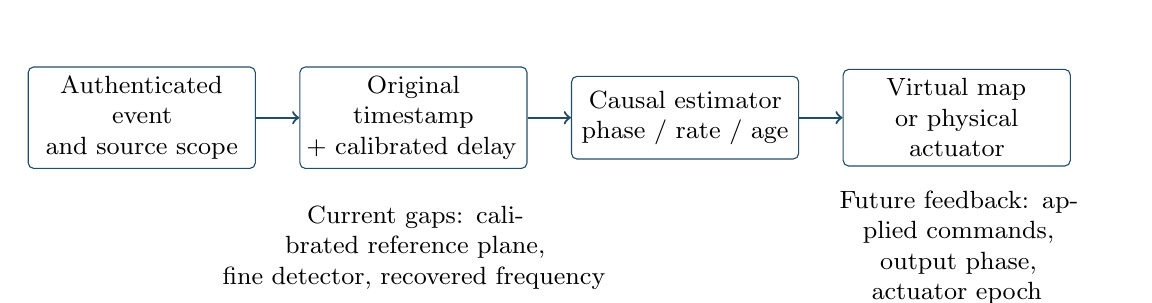
\begin{tikzpicture}[node distance=4mm,box/.style={draw=studyblue,rounded corners=2pt,align=center,font=\small,text width=2.65cm,minimum height=1.05cm},arr/.style={->,thick,studyblue}]
\node[box] (a) at (0,0) {Authenticated event\\and source scope};
\node[box] (b) at (3.45,0) {Original timestamp\\+ calibrated delay};
\node[box] (c) at (6.9,0) {Causal estimator\\phase / rate / age};
\node[box] (d) at (10.35,0) {Virtual map\\or physical actuator};
\draw[arr] (a)--(b);\draw[arr] (b)--(c);\draw[arr] (c)--(d);
\node[align=center,font=\small,text width=5.4cm] at (3.45,-1.65) {Current gaps: calibrated reference plane,\\fine detector, recovered frequency};
\node[align=center,font=\small,text width=4.0cm] at (10.35,-1.65) {Future feedback: applied commands,\\output phase, actuator epoch};
\end{tikzpicture}
\caption{A proposed common architecture. Existing event and authority gates remain prerequisites. The physical-actuator branch and its feedback are future work. This is a design schematic, not a measured signal path.}
\end{figure}

\subsection{Standards and current directions}
The WR Collaboration describes how WR enhancements informed IEEE 1588-2019's High Accuracy Default PTP Profile, including L1 synchronization support, delay asymmetry and timestamp corrections. It also distinguishes the HA protocol from legacy WR-PTP: sharing hardware does not make their protocols interchangeable \cite{ha}. This paper is an architectural comparison; PToB does not thereby implement that profile or acquire IEEE/Bluetooth qualification.

Recent primary material adds several lessons:
\begin{enumerate}
\item \textbf{Servo stages deserve explicit state.} A May 2026 investigation separates reference-clock locking, selection of the second/cycle boundary and fine phase tracking \cite{servo2026}. Our inference is that frequency convergence, epoch alignment and output qualification should remain separately observable.
\item \textbf{The actuator chain and restart state can dominate.} Hu et al.'s June 2026 preprint replaces a DAC/VCXO chain with a Si5345A DSPLL clock generator and implements digital phase control. It separately addresses transceiver alignment after restart and adds temperature feed-forward and cascaded control. The authors report 3.38 ps point-to-point precision over 1 m fiber and 3.92 ps over 50 km \cite{cepc}. These are reported precision metrics for their apparatus, not calibrated absolute UTC accuracy or predictions for BLE. We take the design questions, not their performance numbers or controller gains.
\item \textbf{Calibration must reach an electrical reference plane.} A multi-laboratory WR inter-comparison explicitly relates internal timestamps to external electrical timing terminals \cite{electrical}. Our inference is to identify antenna/RF, detector, counter and output planes before treating a wireless offset as hardware calibration.
\item \textbf{Security and timing can be engineered together.} A May 2026 demonstrator reports PPSi integration with NTS4PTP, peer authentication and replay protection, with initial tests over a 50 km spool \cite{security2026}. This is preliminary demonstrator evidence. It supports keeping authentication in the precision path; it does not establish delay-attack immunity or suggest replacing our enrolled trust model without analysis.
\end{enumerate}

A 2025 holdover presentation describes an expansion-card development program and a projected November 2026 availability date \cite{holdover2025}. That is a dated plan, not confirmation of availability at this paper's cutoff. Its transferable lesson is that holdover is a separately specified output behavior with an oscillator and recovery history, rather than a label inferred from a fitted rate.

\section{What PToB implements today}
Table~\ref{tab:matrix} separates implementation from qualification. References to code mean the exact inspected snapshots in the evidence manifest; runtime history is cited separately.
\small
\begin{longtable}{L{2.5cm}L{5.0cm}L{7.05cm}}
\caption{Implementation comparison and remaining evidence.}\label{tab:matrix}\\
\toprule Mechanism & PToB implementation / retained observation & WR lesson and remaining gap \\
\midrule\endfirsthead
\toprule Mechanism & PToB implementation / retained observation & WR lesson and remaining gap \\
\midrule\endhead
Original-event timestamps & T096 routes RADIO ADDRESS through PPI to TIMER3 capture; selected records retain event/channel, payload and capture scope. & Preserve hardware event identity. The detector's electrical/RF reference point and fixed bias remain separate from callback latency. \\
Two-step correction & A later authenticated correction matches a saved original RX event; completion/availability is distinct from that original tick. & Strong architectural correspondence to two-step time transfer. This alone provides neither calibrated one-way delay nor WR interoperability. \\
Clock estimation & Normal T096 uses a portable causal servo and delivered-map history. RC uses a different rate fit and boundary map. W12 uses a channel-aware fit and corrected map. & Useful software discipline exists. These algorithms are not the WR DDMTD/VCXO loop and do not share one universal lock threshold. \\
Frequency transfer & Packet observations estimate relative counter rate. & BLE packet timing does not expose a continuous recovered SyncE clock. An oscillator actuator would remain packet disciplined unless another reference is provided. \\
Fine physical phase & T096 capture grid is 16 MHz; W12 corrected coordinates use a 20 MHz local basis. & No demonstrated DDMTD, calibrated TDC or RF-carrier phase detector in these paths. Finer numerical time units do not add detector information. \\
Delay correction & The T096 delivered path includes a provisional +10,543 ns per received BLE1M link, trained on a named direct-link PPS population. Raw radio captures remain preserved. & A measured empirical offset is useful engineering evidence. Portability across devices/hops and physical decomposition are unqualified. \\
Authority and lineage & Root/parent boot, source epoch, train/publication/event and original expiry gate consumption. Unknown bounds propagate. & Retain these strengths through any extension. Timing convergence cannot create source authority; authenticated identity alone cannot create an error bound. \\
Relay service & RC maps upstream time and republishes captured downstream timing under admitted lineage. & Functionally resembles boundary-clock time regeneration. It is not demonstrated HA-profile behavior; shared root uncertainty and systematic hop errors remain correlated. \\
Physical actuation & Current inspected paths alter delivered software time. No qualified quartz-pulling or coherent RF actuator is demonstrated. & Future VCXO/DCO/NCO support needs a calibrated plant, applied-command history and measured electrical output. \\
Holdover and recovery & Map age, source expiry, quality and continuity logic exist; regression evidence includes failed reacquisition. & A predicted horizon is distinct from tested blackout output. Stable serving-GM plus authenticated HOT must be restored before broader recovery experiments. \\
USB boundary bridge & TC04 hardware SOF capture is associated with Mac controller frame/time observations; event identity has causal marker checks. & Another example of separating event identity from fitted residual. Source UTC gaps and unknown controller/PHY bias prevent promotion to a qualified host UTC clock. \\
\bottomrule
\end{longtable}
\normalsize

\subsection{Code-level distinctions that matter}
The T096 \code{capture.c} configures a 16 MHz 32-bit TIMER3, allocates PPI resources, captures PPS on CC0 and RADIO ADDRESS on CC1, and optionally captures USB SOF on CC3. \code{radio\_capture.c} associates the selected controller event with a payload and preserves raw ADDRESS alongside its consumer reference. Resource ownership and capture epochs matter as much as numerical resolution \cite{localcode}.

The normal \code{precision\_servo.h} contains a strict 200 ns gate and a separate 1,000 ns experimental attempt gate. Its delivered map applies a 1 ppm phase slew; a generic prediction helper also contains a different 500 ppm slew convention. Conflating those functions would misdescribe the actual delivered clock. RC \code{rc5\_clock\_discipline} instead maintains four immutable maps, uses a one-second continuity slew for small changes, and fences larger discontinuities as unqualified. \code{rc5\_clock\_capture} selects a map effective by the event tick and propagates rate/capture/bias uncertainty with an UNKNOWN sentinel \cite{localcode}.

W12 \code{G1CorrectedClock} retains 64 compact physical observations with 250 ms spacing and separates within-channel rate fitting from all causal quality errors. It scores the previous delivered prediction before the unseen correction can train it. Boot, root, source and parent-path transitions withdraw the applicable scope. The strict capture-provider contract separately requires event/payload association, controller ownership, matching clock/resource incarnations and known calibration bounds; functional reception is not automatically precision-qualified publication \cite{localcode,w12drift}.

These distinctions support a portable estimator/actuator interface, but do not justify silently replacing the three clock paths with one servo. Their units, sign conventions, admission rules and historical evidence must first be reconciled.

\subsection{What the measurements actually establish}
The retained direct T096 calibration has 520 reference-valid causal PPS samples against a nominal 600-edge grid, a raw mean of $-10{,}542.636538\ns$ and demeaned jitter of $51.108\ns$. Applying the chosen $+10{,}543\ns$ to that same training population gives $51.110\ns$ RMS. The 86.67\% calibration coverage, invalid-reference edges and missing intervals remain part of the result. The next 120 s prospective check had zero physical witness PPS edges; it provides no prospective accuracy pass \cite{empirical}. This is not equivalent to an independently calibrated WR electrical time-transfer measurement.

The complete October 12 C2 W12 repair capture reports 1,140 UI records over 570 s, with causal RMS 138--192 ns (median 161 ns). A separate prior-UI prediction analysis reports 160.8 ns RMS; within-channel jitter 160.1 ns dominates the 14.0 ns variation among channel means. The retained report finds no established 100 ns hardware floor and no unique attribution among RX mapping, source jitter and oscillator tracking \cite{w12drift}. Overlapping forecasts and continuously observed packets are not independent blackout tests.

The October 15 USB bridge's 600.008 s replay retains 19,084 hardware tuples and 2,383 valid markers, with 100 inconsistent tuples and 15 markers rejected. A causal previous-window innovation statistic of $0.409\us$ is a bridge diagnostic. Only 248 source samples over about eight seconds and 8/592 source-valid status observations remain. These populations cannot establish ten minutes of usable UTC or a comparison superior to NTP \cite{usb}. No unlike metric in this subsection is pooled with another or ranked against WR's picosecond precision.

\section{Why better oscillators are necessary for some goals, but insufficient}
\subsection{An observation model and its ambiguity}
Use seconds as the unit and define local clock error $x(t)=T_L(t)-T_R(t)$ and fractional frequency error $y=\dot x$. After known nominal event-coordinate conversions, a one-way timestamp observation can be written
\begin{equation}
z_k=x(t_k)+b_{\rm tx}+b_{\rm rx}+d_k+v_k,
\label{eq:oneway}
\end{equation}
where the signed $b$ terms collect endpoint reference-plane offsets under this convention, $d_k$ is propagation and $v_k$ is varying observation error. A constant change in $x$ can be absorbed by the unknown delay sum. Consequently, more packets, a better fit or physical frequency trim cannot uniquely recover absolute phase without another measurement or calibrated assumption.

For a reciprocal four-timestamp exchange, after clock-rate normalization over the exchange,
\begin{align}
t_2-t_1&=x+d_f, & t_4-t_3&=-x+d_r,\\
\widehat x_{\rm sym}&=\tfrac12[(t_2-t_1)-(t_4-t_3)]
=x+\tfrac12(d_f-d_r).
\label{eq:twoway}
\end{align}
Two-way measurement removes common symmetric delay but leaves half the directional asymmetry. This algebra motivates future reciprocal experiments; the current correction path is not thereby a calibrated bidirectional ranging protocol. Wireless directional detector latency, PHY/channel dependence, multipath and antenna geometry require their own reference planes and tests. Optical wavelength-asymmetry coefficients cannot be imported into BLE.

The raw-event investigation already demonstrates the identifiability problem: packet-pair preservation can exclude later processing latency but cannot split the observed bias uniquely among TX/RX detector delay, propagation, source-map phase and independent GPS/PPS delays \cite{rawaudit}. The provisional correction is therefore tagged empirical, not reinterpreted as a measured universal detector constant.

\subsection{Resolution, noise and the meaning of a floor}
A 16 MHz timer has a $62.5\ns$ grid. Under an ideal uniform quantization model, a single error has standard deviation $q/\sqrt{12}=18.04\ns$; the difference of two independent such errors has $q/\sqrt6=25.52\ns$. These are analytical model values, not measured performance or guaranteed bounds. Correlated clock grids, detector latency, signal conditions and mapping errors violate the simple assumptions. Repeated observations can estimate a stable parameter below one tick when they contain suitable phase diversity, but they cannot create a calibrated sub-tick timestamp for an arbitrary individual event.

An actuator chiefly changes frequency evolution, not the precision or absolute bias of the detector. An excellent OCXO can improve holdover while leaving packet phase noise unchanged. A fine TDC can improve event resolution while leaving an unstable oscillator unable to hold phase through a blackout. A synthesizer's low integrated jitter also does not establish antenna-to-output UTC accuracy. The detector, oscillator, servo and reference-plane budget must be evaluated together.

\subsection{A holdover budget that does not renew authority}
For independently justified deterministic bounds at reference loss, a useful candidate model is
\begin{equation}
B_x(h)\le B_0+hB_y+\tfrac12h^2B_{\dot y}+B_{\rm act}(h),
\label{eq:hold}
\end{equation}
where $B_0$ contains phase, path, source and output errors, $B_y$ is fractional-rate uncertainty, $B_{\dot y}$ is drift-rate uncertainty and $B_{\rm act}$ covers quantization/settling/model error of actuation. A stochastic covariance forecast is a different claim and must identify confidence, correlations and model validity. Neither fit RMS nor an estimated rate sigma automatically supplies deterministic bounds.

With an \emph{illustrative} $500\ns$ budget, $100\ns$ initial error, zero drift and no extra actuator error, the remaining $400\ns$ permits rate uncertainty of $200\ppb$ for 2 s, $40\ppb$ for 10 s, $6.67\ppb$ for 60 s or $0.667\ppb$ for 600 s. These calculations are allocations, not new acceptance thresholds or evidence that a present unit satisfies them. Original source and control expiry can terminate permitted service earlier than the physical forecast. Better holdover must never extend those lifetimes implicitly.

\begin{figure}[htbp]
\centering
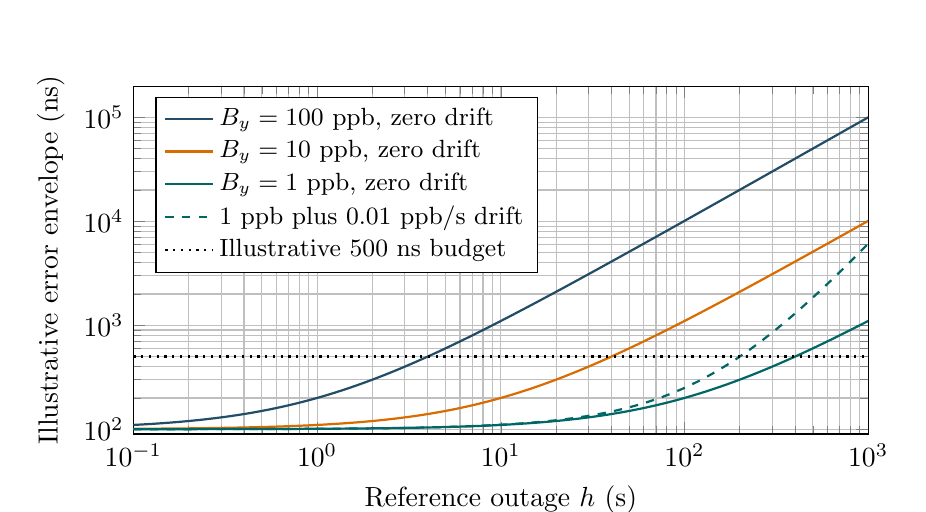
\begin{tikzpicture}
\begin{loglogaxis}[width=.9\linewidth,height=6cm,xlabel={Reference outage $h$ (s)},ylabel={Illustrative error envelope (ns)},xmin=0.1,xmax=1000,ymin=90,ymax=200000,grid=both,legend style={at={(0.03,0.97)},anchor=north west,font=\small},legend cell align=left]
\addplot[studyblue,thick,domain=0.1:1000,samples=100]{100+100*x};\addlegendentry{$B_y=100$ ppb, zero drift}
\addplot[orange!85!black,thick,domain=0.1:1000,samples=100]{100+10*x};\addlegendentry{$B_y=10$ ppb, zero drift}
\addplot[teal!80!black,thick,domain=0.1:1000,samples=100]{100+x};\addlegendentry{$B_y=1$ ppb, zero drift}
\addplot[teal!80!black,dashed,thick,domain=0.1:1000,samples=100]{100+x+0.005*x*x};\addlegendentry{$1$ ppb plus $0.01$ ppb/s drift}
\addplot[black,dotted,thick,domain=0.1:1000]{500};\addlegendentry{Illustrative 500 ns budget}
\end{loglogaxis}
\end{tikzpicture}
\caption{Analytical examples from Eq.~\ref{eq:hold}; no experimental points or fitted device parameters. Assumed $B_0=100$ ns and $B_{\rm act}=0$. A good initial rate estimate alone cannot remove long-term drift. Source authority and physical error are separate gates.}
\end{figure}

\section{A proposed protocol and control extension}
\subsection{Keep transport, estimation and actuation separate}
We propose a bounded local interface with four stages: capture an immutable original; authenticate and admit its correction under the unchanged scope; estimate phase/rate at an explicit event and command time; apply either a virtual-map update or a supported physical command. No new message layout, codepoint or routine RF traffic is approved by this paper. Existing public GM announcements and boot defaults remain intact.

A future optional negotiated profile could carry the following concepts, with exact units, ranges, sentinels and golden vectors defined before implementation:
\begin{enumerate}
\item \textbf{Measurement profile:} detector kind, event/reference plane, counter scale, PHY/channel class, calibration ID and revision, validity conditions, temperature range, uncertainty kind and correlation group.
\item \textbf{Clock and actuator capability:} virtual map, adjustable divider/NCO, external tunable oscillator, DCO synthesizer or recovered reference; tuning sign/range/resolution, update interval, settling model, phase-step support and safe fallback.
\item \textbf{Applied state:} clock/actuator incarnation, acknowledged command sequence, requested versus applied value, application time, saturation/fault flags and output-valid state. Local detailed telemetry may suffice; peer traffic should be added only for demonstrated need.
\item \textbf{Quality:} separately reported algorithm convergence, frequency lock, epoch alignment, phase tracking, holdover forecast and qualified output. A calibration flag must identify what was calibrated rather than grant blanket precision.
\end{enumerate}
Missing or unsupported capabilities remain explicit. A legacy peer continues its existing profile; a new profile must be negotiated or refused, never inferred from packet length or a familiar device identity. An authenticated capability report still requires local proof that the declared actuator and calibration are applicable.

\subsection{A causal estimator with actuator accounting}
For irregular intervals $\Delta_k$, let $y_{\rm free}$ be the oscillator's fractional-rate error before actuator correction. A candidate state $s=[x,y_{\rm free},\dot y_{\rm free}]^\mathrm T$ evolves under
\begin{equation}
s_{k+1}=\begin{bmatrix}1&\Delta_k&\Delta_k^2/2\\0&1&\Delta_k\\0&0&1\end{bmatrix}s_k+
\begin{bmatrix}\Delta_k\\0\\0\end{bmatrix}g_k u_k+w_k,
\label{eq:plant}
\end{equation}
for an absolute command held over the interval with calibrated fractional-rate effect $g_ku_k$. Thus $\dot x=y_{\rm free}+gu$: the actuator changes total rate while the state retains the underlying free-running oscillator rate. This simplified memoryless plant excludes settling; measured plant dynamics and multiple command changes require additional state or explicit subinterval integration. The later PI equation uses a command already expressed in fractional-frequency units, so its calibrated gain is absorbed into that command.

The input history must contain commands actually applied, not merely requested. Observations belong at $t_k$ even if authenticated availability is later at $a_k$. A candidate estimator may update a bounded past state and propagate it forward using retained inputs, or use an equivalent delayed-measurement formulation. It cannot retroactively improve a previously delivered map or score a newly trained model as a prior prediction. W12's pre-update causal scoring is a useful existing pattern \cite{localcode}.

For a simple negative-feedback convention with $e=\widehat T_L-\widehat T_R$ in seconds and positive actuator gain increasing local frequency, a candidate control law is
\begin{equation}
I_{k+1}=I_k+e_k\Delta_k,\qquad
u_k=\operatorname{clip}[-K_p e_k-K_i I_k-\widehat y_{\rm free},u_{\min},u_{\max}].
\label{eq:pi}
\end{equation}
Here $u$ is commanded fractional frequency, $K_p$ has units $\mathrm{s}^{-1}$ and $K_i$ has units $\mathrm{s}^{-2}$. Estimated $y_{\rm free}$ must exclude the already applied actuator correction; otherwise feed-forward double-counts it. This equation defines signs and units, not tuned gains. Add anti-windup, slew/range clamps, command acknowledgement, numerical checks and bumpless acquisition/holdover transitions. Identify an internal synthesizer loop before selecting an outer-loop bandwidth. Tune to measured oscillator and packet-noise spectra, not a borrowed WR constant.

\subsection{A tunable measurement counter changes the mapping problem}
If the actuator steers the same oscillator that clocks the capture counter, its ticks no longer represent one fixed nominal period plus a single constant slope across arbitrary command changes. Preserve the monotonically extended raw count and its incarnation, but use piecewise mappings with command application times and uncertainty. Never reset or rewrite the capture counter to hide a phase error. If only a separate output synthesizer is steered, keep the original counter as an observation reference and model that output's relation to it explicitly.

Likewise, a trim command that reaches the MCU clock need not reach its radio PLL, output divider or peripheral clock. A future target must document the clock tree. Frequency lock does not align a PPS divider's epoch, and a programmable RF synthesizer does not establish carrier coherence without a suitable phase observation and calibrated signal path.

\section{Hardware options and measurable research priorities}
\small
\begin{longtable}{L{3.0cm}L{5.5cm}L{6.05cm}}
\caption{Candidate target capabilities; no component purchase or performance guarantee is implied.}\\
\toprule Target capability & Expected contribution & Prerequisite / limitation \\
\midrule\endfirsthead
\toprule Target capability & Expected contribution & Prerequisite / limitation \\
\midrule\endhead
Current fixed quartz + virtual map & Better estimator freshness, causal accounting, path diagnostics and software-delivered time. & Leaves physical oscillator unsteered; output scheduling resolution and calibration still matter. \\
TCXO/OCXO with supported trim & Lower free-running drift and potentially longer holdover; physical frequency control if actually exposed. & Measure tuning polarity/gain, warm-up, aging, thermal behavior, power and phase noise. Stability grade alone does not provide an actuator. \\
External DAC + VCXO & Direct analog frequency actuation and possible phase steering through a servo. & DAC noise/resolution, tuning nonlinearity, supply noise, loop stability and safe rail limits need calibration. \\
DCO/DSPLL synthesizer & Digital frequency/phase commands and configurable clock distribution. & Command timing, phase continuity, internal loop dynamics and restart determinism must be tested. Fine command granularity is not output accuracy. \\
FPGA + TDC or DDMTD & Finer event or periodic-clock phase observation; hardware scheduling opportunities. & DDMTD needs suitable accessible clocks, not just packet interrupts. Calibrate detector nonlinearity, temperature and reference plane. \\
WR endpoint or gateway & A calibrated wired reference can anchor or witness a wireless experiment. & A calibrated WR input does not remove the wireless last-hop uncertainty. Gateway boundary uncertainty must propagate. \\
\bottomrule
\end{longtable}
\normalsize

We recommend three ordered research stages. \textbf{Stage A uses retained evidence and models.} Audit original-event identity and units across the GM, RC and W12 paths; replay delay, stale-fit, source-change and command-saturation cases; decompose the error budget; and specify the capability/calibration contract. Establish the GM/HOT recovery milestone in its separately authorized work before scheduling dependent live recovery studies. This paper does not implement that work.

\textbf{Stage B characterizes reference planes and the target plant.} Under a future authorized hardware plan, use a calibrated common-edge or time-interval reference, record instrument/cable uncertainty, and measure each board/direction/PHY/channel and received-signal condition. Train empirical terms on one population and validate on separately frozen devices, restarts, temperature intervals and link conditions. Characterize frequency trim with controlled steps and record the actual application edge. Verify electrical PPS/divider alignment independently of the packet estimator. Use WR as a witness only when its own output and path calibration are documented.

\textbf{Stage C compares disciplined outputs prospectively.} Freeze a virtual-map baseline and a physical-actuation candidate; use the same reference plane and observer budget. Compare acquisition, steady tracking, temperature/power changes, genuine reference blackouts, source/parent restarts, link loss, scope changes, saturation and failover. Study update-rate reduction only after maintaining the same error, authority and recovery requirements. Better oscillator stability is a reason to test lower radio duty, not evidence of energy savings. Include CPU, memory, actual RX residence, RF airtime, power and logger drops.

For each case, report signed bias, undetrended RMS, demeaned jitter, P95/P99/max absolute error, duration, valid/expected coverage, all gaps, startup/recovery exclusions and retained failures. Add TIE, phase-noise spectra, ADEV/MDEV/TDEV where the sampling and reference support them; do not invent evenly spaced data across outages. Report repeated-restart offsets separately from within-run jitter. Pairwise nodes sharing a GM are correlated witnesses, so a residual cannot be divided by hop count or $\sqrt N$ to obtain measured per-hop accuracy. Authentication should be tested against replay and delay manipulation while preserving original expiry; cryptographic validity is not freshness of the physical event by itself.

\section{Discussion and defensible contribution}
PToB's strongest present correspondence to precision timing practice is its insistence on preserved physical events, causal correction availability and source lineage. Those mechanisms are useful across hardware generations. Its present empirical offset, fitted oscillator rate and lock displays do not yet establish a calibrated antenna-to-output clock, physically disciplined quartz or a deterministic blackout error bound. The October 15 regressions further show that source admission and serving continuity can dominate usefulness even when the local timestamp machinery is precise.

The most useful immediate deliverable is therefore a common description of measurement planes, calibration validity, clock capabilities and applied actuation, together with reproducible causal evaluation. A future tunable target should close a measured error budget and demonstrate electrical output through restarts and reference outages. Claims of wireless novelty, energy reduction, WR compatibility, sub-nanosecond accuracy, carrier coherence or superiority to NTP require their own evidence and broader prior-art review.

A plausible future paper contribution is a controller-respecting, authenticated wireless timing architecture that can use heterogeneous virtual and physical clock actuators while retaining causal event provenance and honest uncertainty. This draft establishes the comparison and research questions. It does not claim that the proposed extension has been built or validated.

\section*{Reproducibility and disclosure}
The companion \path{white-rabbit-study-evidence-20261015.json} maps claims to exact source/report hashes and retained local input snapshots. \path{provenance/white-rabbit-literature-20261015.json} records URLs, publication context, access limits and the claims taken from each external source. The build manifest identifies compiler, source, PDF and render checks. Local copies and hashes establish reproducibility and identity, not calibration, durable external backup or public data availability. Original private raw captures were not republished or reanalyzed for new measurements.

OpenAI Codex assisted literature retrieval, source inspection, analysis, equations, drafting and document preparation. Jonathan Yantis is the proposed human author and must review the claims before submission. This local research draft has not been submitted or peer reviewed.

\begin{thebibliography}{99}
\raggedright
\bibitem{wr2011} M. Lipinski, T. Wlostowski, J. Serrano and P. Alvarez, ``White Rabbit: a PTP Application for Robust Sub-nanosecond Synchronization,'' ISPCS, 2011. \url{https://white-rabbit.web.cern.ch/documents/White_Rabbit-a_PTP_application_for_robust_sub-nanosecond_synchronization.pdf}.
\bibitem{characteristics} M. Rizzi et al., ``White Rabbit clock characteristics,'' ISPCS, 2016, doi:10.1109/ISPCS.2016.7579514. \url{https://white-rabbit.web.cern.ch/documents/White_Rabbit_Clock_Characteristics.pdf}.
\bibitem{ha} White Rabbit Collaboration, ``IEEE1588 Standard,'' checked 15 October 2026. \url{https://white-rabbit-collaboration-website.web.cern.ch/ieee1588-standard/}. This is the Collaboration's standards explanation, not a claim to have audited the full normative standard.
\bibitem{servo2026} K. Asteriou, ``Analysis of Sub-Optimal Servo Performance in White Rabbit Timing Systems,'' 15th White Rabbit Workshop, 27 May 2026, abstract and CERN recording metadata/indexed transcript. \url{https://indico.cern.ch/event/1623507/contributions/7073395/}; \url{https://videos.cern.ch/record/3025754}.
\bibitem{cepc} J. Hu, X. Zhou, X. Jiang and D. Jin, ``A High-Precision Clock Synchronization System for the CEPC Accelerator,'' arXiv:2606.11590v1, 10 June 2026, preprint. \url{https://arxiv.org/abs/2606.11590}.
\bibitem{electrical} P. P. M. Jansweijer et al., ``First electrical White Rabbit absolute calibration inter-comparison,'' arXiv:2201.08640v1, 21 January 2022. \url{https://arxiv.org/abs/2201.08640}.
\bibitem{security2026} D. Chung, ``Cryptographically Secured High-Performance Time Synchronization for White Rabbit Links,'' 15th White Rabbit Workshop, 27 May 2026, indexed primary abstract. \url{https://indico.cern.ch/event/1623507/contributions/7073396/}.
\bibitem{holdover2025} D. Chung and N. Amey, ``Adding relevant holdover capability to the WRS v4,'' 14th White Rabbit Workshop, 26 June 2025, development update. \url{https://indico.cern.ch/event/1524513/contributions/6556224/}.
\bibitem{localcode} PToB project, inspected code snapshots, 15 October 2026: T096 \code{v12\_r2/src/capture.c}, \code{radio\_capture.c}, \code{rc\_boundary.c}, \code{include/precision\_servo.h}, \code{rc\_direct\_calibration.h}; W12 \code{v12\_native/main/g1\_corrected\_clock.hpp} and \code{capture\_contract.hpp}. Exact SHA-256 hashes and function/claim mappings are in the companion evidence manifest. Source snapshots are not installed-image attestations.
\bibitem{empirical} PToB project, \code{docs/RC\_EMPIRICAL\_OFFSET\_AND\_NEXT\_HOP\_20261012.md}, 12 October 2026. Training/validation populations and limits retained separately.
\bibitem{w12drift} PToB project, \code{docs/W12\_C2\_DRIFT\_FIX\_20261012.md} and matching JSON result, 12 October 2026.
\bibitem{rawaudit} PToB project, \code{docs/RC\_TIMESTAMP\_RAW\_INVESTIGATION\_20261012.md}, 12 October 2026.
\bibitem{usb} PToB project, \code{results/T096\_USB\_BOUNDARY\_MAPPING\_20261015.json} and \code{docs/T096\_USB\_FRAME\_BRIDGE\_20261015.md}, 15 October 2026.
\bibitem{regression} PToB project, \code{docs/T096\_048\_REGRESSION\_INVESTIGATION\_20261015.md}, matching investigation JSON and \code{results/T096\_COHORT\_RELEASE\_20261015.json}, 15 October 2026. Release rejected; restart recovery does not establish a durable fix.
\end{thebibliography}
\end{document}
